\documentclass[12pt,a4paper,openright]{report}

\usepackage[a4paper,margin=2.5cm]{geometry}
\usepackage{fontspec}
\usepackage{polyglossia}
\setmainlanguage{vietnamese}
\setotherlanguage{english}
\usepackage{graphicx}
\usepackage{booktabs}
\usepackage{array}
\usepackage{hyperref}
\hypersetup{
  colorlinks=true,
  linkcolor=black,
  urlcolor=blue,
  pdftitle={Luận văn thạc sĩ}
}

\newcommand{\university}{Tên trường đại học}
\newcommand{\faculty}{Tên khoa}
\newcommand{\department}{Tên bộ môn}
\newcommand{\program}{Chương trình thạc sĩ}
\newcommand{\thesistitle}{Tên luận văn thạc sĩ}
\newcommand{\studentname}{Họ và tên học viên}
\newcommand{\studentid}{Mã số học viên}
\newcommand{\supervisor}{Giảng viên hướng dẫn}
\newcommand{\submissionplace}{Thành phố Hồ Chí Minh}

\begin{document}

\pagenumbering{roman}

\begin{titlepage}
  \centering
  {\Large \university\par}
  \vspace{0.25cm}
  {\large \faculty\par}
  \vspace{0.15cm}
  {\large \department\par}
  \vfill
  {\Large \bfseries LUẬN VĂN THẠC SĨ\par}
  \vspace{0.8cm}
  {\LARGE \bfseries \thesistitle\par}
  \vspace{1.2cm}
  \begin{flushleft}
    \large
    Học viên: \studentname\\
    Mã số: \studentid\\
    Chương trình: \program\\
    Giảng viên hướng dẫn: \supervisor
  \end{flushleft}
  \vfill
  {\large \submissionplace, \the\year\par}
\end{titlepage}

\chapter*{Lời cam đoan}
\addcontentsline{toc}{chapter}{Lời cam đoan}
Nội dung cam đoan của học viên.

\chapter*{Lời cảm ơn}
\addcontentsline{toc}{chapter}{Lời cảm ơn}
Nội dung lời cảm ơn.

\chapter*{Tóm tắt}
\addcontentsline{toc}{chapter}{Tóm tắt}
Tóm tắt ngắn gọn mục tiêu, phương pháp, kết quả và đóng góp chính của luận văn.

\chapter*{Abstract}
\addcontentsline{toc}{chapter}{Abstract}
Short English abstract of the thesis.

\tableofcontents
\listoffigures
\listoftables
\clearpage

\pagenumbering{arabic}
\chapter{Giới thiệu}

\section{Bối cảnh}
Trình bày bối cảnh và lý do chọn đề tài.

\section{Mục tiêu}
Nêu mục tiêu nghiên cứu của luận văn.

\section{Phạm vi}
Xác định phạm vi thực hiện và các giới hạn của đề tài.

\chapter{Tổng quan tài liệu}

\section{Bối cảnh nghiên cứu}
Mô tả các hướng nghiên cứu liên quan.

\section{Khoảng trống nghiên cứu}
Nêu vấn đề chưa được giải quyết đầy đủ trong tài liệu hiện có.

\chapter{Vật liệu và phương pháp nghiên cứu}

\section{Hóa chất, thiết bị và dụng cụ}
\subsection{Hóa chất}
\begin{table}[htbp]
\centering
\small
\caption{Danh mục hóa chất sử dụng}
\label{tab:chemicals}
\begin{tabular}{@{}c>{\raggedright\arraybackslash}p{3.1cm}>{\raggedright\arraybackslash}p{5.6cm}>{\raggedright\arraybackslash}p{3.0cm}@{}}
\toprule
STT & Tên hóa chất & Nơi sản xuất/Nhà sản xuất & Chỉ số/Cấp thuốc thử \\
\midrule
1 & Glycerol (C$_3$H$_8$O$_3$) & Fisher Chemical & 99+\%, Analytical Reagent \\
2 & Polyvinyl\-pyrrolidone K30 (PVP K30) & HiMedia Laboratories, India & K30 \\
3 & Carboxymethyl cellulose (CMC) & FUJIFILM Wako Pure Chemical Corporation, Japan & Reagent \\
4 & Sodium hydroxide (NaOH) & Xilong Scientific Co., Ltd., China & Analytical Reagent (AR) \\
5 & Silver nitrate (AgNO$_3$) & Xilong Scientific Co., Ltd., China & 99\% \\
\bottomrule
\end{tabular}
\end{table}

\section{Quy trình tổng hợp AgNPs}
\subsection{Chuẩn bị dung dịch}
AgNPs được tổng hợp bằng phương pháp polyol, trong đó glycerol được sử dụng làm môi trường phản ứng.
Hai hệ tổng hợp được khảo sát gồm hệ Ag@PVP sử dụng polyvinyl\-pyrrolidone (PVP) làm chất bảo vệ không ion và hệ Ag@CMC sử dụng carboxymethyl cellulose (CMC) làm chất bảo vệ mang điện tích âm.
Dung dịch tiền chất AgNO$_3$ và glycerol được sử dụng chung cho hai hệ, trong khi chất bảo vệ, điều kiện kiềm và thời gian phản ứng được thiết lập riêng cho từng hệ.

\textbf{Dung dịch AgNO$_3$ 10mM}: Cân chính xác 0,1700 g AgNO$_3$, hòa tan hoàn toàn trong nước cất, chuyển dung dịch vào bình định mức 100 mL và bổ sung nước đến vạch mức. 

\textbf{Dung dịch PVP 2\% w/v}: Hòa tan 2,00 g PVP trong nước cất dưới khuấy từ đến khi thu được dung dịch đồng nhất, chuyển dung dịch vào bình định mức 100 mL và bổ sung nước đến vạch mức.

\textbf{Dung dịch CMC 3\% w/v}: Hoà tan 0,300 g CMC trong lượng nước thích hợp, sau đó khuấy kết hợp gia nhiệt ở 60~$^\circ$C để thúc đẩy quá trình hydrat hóa và hòa tan polymer. 
Sau khi CMC được phân tán đồng nhất, chuyển dung dịch vào bình định mức 100 mL và bổ sung nước đến vạch mức.
Dung dịch CMC được để qua đêm trước khi sử dụng để quá trình hydrat hóa polymer diễn ra đầy đủ và hệ đạt trạng thái đồng nhất.

\textbf{Dung dịch NaOH}: Đối với hệ Ag@PVP, hòa tan 0,0300 g NaOH trong nước cất và định mức đến 50 mL để thu dung dịch NaOH 15 mM.
Đối với hệ Ag@CMC, hòa tan 0,0400 g NaOH trong nước cất và định mức đến 50 mL để thu dung dịch NaOH 20 mM.


\subsection{Quy trình tổng hợp hệ Ag@PVP}
Hạt nano bạc được tổng hợp trong hệ glycerol–nước với PVP đóng vai trò chất bảo vệ. 
Trước tiên, cho 6 mL glycerol, 1 mL dung dịch PVP 2\% (w/v) và 1 mL dung dịch NaOH 15 mM vào bình phản ứng. 
Tiếp theo, bổ sung 1 mL nước cất để tổng thể tích dung dịch nền đạt 9 mL. 
Hỗn hợp được trộn đều nhằm đảm bảo sự phân bố đồng nhất của các thành phần trong hệ phản ứng.

Dung dịch nền sau đó được đặt trong bể ổn nhiệt và gia nhiệt trong khoảng 5 phút đến khi đạt nhiệt độ đạt 60~$^\circ$C. 
Khi nhiệt độ của hệ đã ổn định, 1 mL dung dịch AgNO$_3$ 10 mM được bổ sung từ từ vào bình phản ứng dưới điều kiện khuấy liên tục nhằm hạn chế sự thay đổi nồng độ cục bộ và tạo điều kiện cho quá trình hình thành hạt diễn ra đồng đều.

Sau khi thêm hoàn toàn dung dịch AgNO$_3$, phản ứng được tiếp tục duy trì ở 60~$^\circ$C trong 30 phút dưới điều kiện khuấy ổn định.

\subsection{Quy trình tổng hợp hệ Ag@CMC}
Hạt nano bạc được tổng hợp trong hệ glycerol–nước với CMC đóng vai trò chất bảo vệ. 
Trước tiên, cho 6 mL glycerol, 1 mL dung dịch CMC 0,3\% (w/v) và 1 mL dung dịch NaOH 20 mM vào bình phản ứng. 
Tiếp theo, bổ sung 1 mL nước cất để tổng thể tích dung dịch nền đạt 9 mL. 
Hỗn hợp được trộn đều nhằm đảm bảo sự phân bố đồng nhất của các thành phần trong hệ phản ứng.

Dung dịch nền sau đó được đặt trong bể ổn nhiệt và gia nhiệt trong khoảng 5 phút đến khi đạt nhiệt độ đạt 60~$^\circ$C. 
Khi nhiệt độ của hệ đã ổn định, 1 mL dung dịch AgNO$_3$ 10 mM được bổ sung từ từ vào bình phản ứng dưới điều kiện khuấy liên tục nhằm hạn chế sự thay đổi nồng độ cục bộ và tạo điều kiện cho quá trình hình thành hạt diễn ra đồng đều.

Sau khi thêm hoàn toàn dung dịch AgNO$_3$, phản ứng được tiếp tục duy trì ở 60~$^\circ$C trong 15 phút dưới điều kiện khuấy ổn định.

\section{Thiết kế khảo sát và tối ưu hóa quá trình tổng hợp AgNPs}
Để xác định điều kiện thích hợp cho quá trình tổng hợp AgNPs trong hai hệ bảo vệ PVP và CMC, nghiên cứu kết hợp phương pháp khảo sát đơn yếu tố (OFAT) với phương pháp mô hình hóa bề mặt đáp ứng (RSM).
Việc kết hợp hai cách tiếp cận nhằm tận dụng ưu điểm của từng phương pháp trong các giai đoạn khác nhau của quá trình tối ưu hóa.

Cách tiếp cận kết hợp này cho phép quá trình tối ưu hóa được thực hiện theo hai cấp độ.
OFAT được sử dụng để khảo sát và thu hẹp không gian thực nghiệm, trong khi RSM được sử dụng để đánh giá hệ trong không gian đa biến và xác định điều kiện tối ưu dựa trên mô hình thống kê.
Do đó, kết quả cuối cùng không chỉ cung cấp một công thức tổng hợp phù hợp mà còn cho phép đánh giá mối quan hệ giữa các thông số phản ứng và sự hình thành AgNPs trong từng hệ bảo vệ.

\subsection{Tối ưu hóa một yếu tố đối với hệ Ag@PVP}
Sau khi xây dựng quy trình tổng hợp ban đầu, phương pháp OFAT được sử dụng để khảo sát ảnh hưởng riêng lẻ của các thông số phản ứng đến quá trình hình thành AgNPs trong hệ Ag@PVP.
Năm yếu tố được khảo sát lần lượt gồm tỷ lệ glycerol, nồng độ NaOH, nhiệt độ phản ứng, thời gian phản ứng và nồng độ PVP.

Sau mỗi thí nghiệm, sản phẩm AgNPs được đánh giá sơ bộ bằng máy quảng phổ UV-Vis sao cho giá trị bước sóng đo được là nhỏ nhất đồng thời độ hấp thụ là lớn nhất nhằm xác định điều kiện tạo hệ tốt nhất.
Giá trị được lựa chọn từ mỗi bước OFAT được sử dụng làm điều kiện cố định cho bước khảo sát tiếp theo.

\subsubsection{Khảo sát ảnh hưởng của tỷ lệ glycerol}
Ảnh hưởng của hàm lượng glycerol trong môi trường phản ứng đến quá trình hình thành AgNPs được khảo sát tại các mức 30, 40, 50, 60 và 70\% (v/v). 
Trong từng thí nghiệm, tỷ lệ glycerol được thay đổi bằng cách điều chỉnh tương ứng thể tích glycerol và nước, trong khi nồng độ AgNO$_3$, hàm lượng PVP, nồng độ NaOH, nhiệt độ và thời gian phản ứng được giữ cố định theo điều kiện cơ sở nhằm đảm bảo nguyên tắc khảo sát một yếu tố tại một thời điểm (OFAT).

Khảo sát này được thực hiện nhằm đánh giá ảnh hưởng của thành phần dung môi glycerol–nước đến quá trình hình thành và đặc tính quang học của AgNPs, thông qua sự thay đổi của các thông số đặc trưng trên phổ UV–Vis. 
Trên cơ sở kết quả thu được, tỷ lệ glycerol cho đáp ứng phù hợp nhất được lựa chọn làm điều kiện cố định cho các thí nghiệm khảo sát tiếp theo.

\subsubsection{Khảo sát ảnh hưởng của nồng độ NaOH}
Sau khi xác định được tỷ lệ glycerol thích hợp, ảnh hưởng của nồng độ NaOH đến quá trình hình thành AgNPs trong hệ Ag@PVP được khảo sát trong khoảng 0–3,0 mM, tại các mức 0; 0,5; 1,0; 1,5; 2,0; 2,5 và 3,0 mM.

Trong quá trình khảo sát, tỷ lệ glycerol được cố định tại giá trị đã lựa chọn từ thí nghiệm trước, trong khi nồng độ AgNO$_3$, hàm lượng PVP, nhiệt độ và thời gian phản ứng được duy trì không đổi theo điều kiện cơ sở. 
Việc thay đổi riêng nồng độ NaOH cho phép đánh giá ảnh hưởng của môi trường kiềm đến quá trình khử ion Ag$^+$, hình thành mầm và phát triển AgNPs trong hệ phản ứng.

Các mẫu sau phản ứng được phân tích dựa trên đặc trưng phổ UV–Vis nhằm xác định sự thay đổi của đáp ứng quang học theo nồng độ NaOH. 
Trên cơ sở kết quả thu được, nồng độ NaOH thích hợp được lựa chọn và sử dụng làm điều kiện cố định cho các khảo sát tiếp theo của hệ Ag@PVP.

\subsubsection{Khảo sát ảnh hưởng của nhiệt độ phản ứng}
Ảnh hưởng của nhiệt độ phản ứng đến quá trình hình thành AgNPs được khảo sát tại năm mức nhiệt độ, lần lượt là 40, 50, 60, 70 và 80 $^\circ$C. 
Trong quá trình khảo sát, tỷ lệ glycerol và nồng độ NaOH được cố định tại các giá trị thích hợp đã xác định từ hai bước khảo sát trước. 
Các thông số phản ứng còn lại được duy trì không đổi nhằm đảm bảo sự thay đổi của đáp ứng thu được chủ yếu phản ánh ảnh hưởng của nhiệt độ.

Kết quả khảo sát được sử dụng để đánh giá sự thay đổi của quá trình hình thành AgNPs theo nhiệt độ, đồng thời xác định khoảng nhiệt độ phù hợp cho hệ phản ứng. 
Giá trị nhiệt độ tương ứng với đáp ứng mong muốn được lựa chọn làm điều kiện khảo sát cố định cho các bước tối ưu hóa tiếp theo.

\subsubsection{Khảo sát ảnh hưởng của thời gian phản ứng}
Sau khi xác định được các điều kiện thích hợp về tỷ lệ glycerol, nồng độ NaOH và nhiệt độ phản ứng, ảnh hưởng của thời gian phản ứng đến quá trình hình thành AgNPs được khảo sát trong khoảng 0–35 phút, với bước khảo sát 5 phút. 
Các thời điểm khảo sát lần lượt là 0, 5, 10, 15, 20, 25, 30 và 35 phút.

Trong quá trình khảo sát, các thông số đã được xác định từ các bước trước được giữ cố định, bao gồm tỷ lệ glycerol, nồng độ NaOH và nhiệt độ phản ứng. 
Nồng độ PVP cũng được duy trì không đổi trong toàn bộ thí nghiệm. 
Việc kiểm soát các thông số này nhằm đánh giá riêng ảnh hưởng của thời gian phản ứng đến quá trình hình thành và đặc tính quang học của AgNPs, từ đó xác định thời gian phản ứng thích hợp cho các bước tối ưu hóa tiếp theo.

\subsubsection{Khảo sát ảnh hưởng của nồng độ PVP}
Sau khi xác định được các điều kiện thích hợp về tỷ lệ glycerol, nồng độ NaOH, nhiệt độ và thời gian phản ứng, ảnh hưởng của nồng độ PVP đến quá trình tổng hợp AgNPs được khảo sát tại các mức 0; 1; 2; 3 và 4\% (w/v).

Trong quá trình khảo sát, toàn bộ các thông số phản ứng khác được giữ cố định tại các giá trị thích hợp đã xác định từ các bước khảo sát trước, nhằm đảm bảo đánh giá riêng ảnh hưởng của nồng độ PVP đến quá trình hình thành và ổn định hệ AgNPs.

Mức 0\% (w/v) được đưa vào thiết kế khảo sát như một mẫu đối chứng không sử dụng chất bảo vệ, qua đó làm cơ sở đánh giá vai trò của PVP đối với sự hình thành, ổn định và đặc tính quang học của AgNPs.

Kết quả khảo sát nồng độ PVP được kết hợp với kết quả của các bước OFAT trước đó để xác định điều kiện tối ưu sơ bộ của hệ Ag@PVP. 
Đây là cơ sở để lựa chọn và thiết lập vùng khảo sát cho thiết kế RSM ở giai đoạn tiếp theo.

\begin{table}[htbp]
\centering
\caption{Trình tự và điều kiện khảo sát OFAT đối với hệ Ag@PVP}
\label{tab:ofat-ag-pvp}
\begin{tabular}{@{}clp{5.0cm}p{5.0cm}@{}}
\toprule
Giai đoạn & Yếu tố khảo sát & Mức khảo sát & Các yếu tố còn lại \\
\midrule
1 & Glycerol & 30, 40, 50, 60, 70\% (v/v) & Giữ cố định \\
2 & NaOH & 0--3,0 mM; bước 0,5 mM & Glycerol thích hợp và các yếu tố khác cố định \\
3 & Nhiệt độ & 40, 50, 60, 70, 80~$^\circ$C & Glycerol và NaOH thích hợp \\
4 & Thời gian & 0--35 phút; bước 5 phút & Glycerol, NaOH và nhiệt độ thích hợp; PVP cố định \\
5 & PVP & 0, 1, 2, 3, 4\% (w/v) & Các yếu tố còn lại tại điều kiện thích hợp \\
\bottomrule
\end{tabular}
\end{table}

\subsection{Tối ưu hóa một yếu tố đối với hệ Ag@CMC}
Quá trình khảo sát đơn yếu tố đối với hệ Ag@CMC được thực hiện theo trình tự: tỷ lệ glycerol, nồng độ NaOH, nhiệt độ, thời gian phản ứng và nồng độ CMC.
Sau mỗi bước khảo sát, điều kiện cho đáp ứng tốt nhất được lựa chọn và sử dụng làm điều kiện cố định cho bước khảo sát tiếp theo.
Các yếu tố được khảo sát theo cùng một trình tự với hệ PVP nhằm xác định xu hướng ảnh hưởng của từng thông số đối với hệ.
Các thông số không được khảo sát trong từng thí nghiệm được giữ nguyên theo quy trình tổng hợp cơ sở được trình bày ở Mục~3.2.

\subsubsection{Khảo sát ảnh hưởng của tỷ lệ glycerol}
Ảnh hưởng của tỷ lệ glycerol trong môi trường phản ứng được khảo sát tại các mức 40, 50, 60 và 70\% (v/v).
Các thông số khác được giữ cố định theo điều kiện tổng hợp cơ sở.

\subsubsection{Khảo sát ảnh hưởng của nồng độ NaOH}
Sau khi xác định được tỷ lệ glycerol thích hợp, ảnh hưởng của nồng độ NaOH được khảo sát tại các mức 0, 1, 2, 3 và 4 mM.
Trong mỗi thí nghiệm, tỷ lệ glycerol được giữ tại giá trị được lựa chọn từ bước trước, trong khi các thông số còn lại được duy trì không đổi.
Kết quả được sử dụng để xác định nồng độ NaOH thích hợp đối với quá trình hình thành AgNPs trong hệ Ag@CMC.

\subsubsection{Khảo sát ảnh hưởng của nhiệt độ phản ứng}
Ảnh hưởng của nhiệt độ phản ứng được khảo sát tại 40, 50, 60, 70 và 80~$^\circ$C.
Tỷ lệ glycerol và nồng độ NaOH được cố định tại các giá trị thích hợp được xác định từ hai bước khảo sát trước đó; các thông số còn lại được giữ nguyên.

Kết quả khảo sát được sử dụng để xác định nhiệt độ phản ứng thích hợp cho các bước tối ưu hoá tiếp theo.

\subsubsection{Khảo sát ảnh hưởng của thời gian phản ứng}
Sau khi xác định được tỷ lệ glycerol, nồng độ NaOH và nhiệt độ thích hợp, ảnh hưởng của thời gian phản ứng được khảo sát tại các thời điểm 0, 5, 10, 15, 20, 25 và 30 phút.

Thời gian phản ứng được tính từ thời điểm hoàn tất quá trình thêm dung dịch AgNO$_3$ vào hệ phản ứng.
Các thông số còn lại được cố định tại các giá trị được lựa chọn từ các bước khảo sát trước.
Nồng độ CMC được giữ cố định trong toàn bộ quá trình khảo sát thời gian.

Kết quả được sử dụng để xác định thời gian phản ứng thích hợp đối với hệ Ag@CMC.

\subsubsection{Khảo sát ảnh hưởng của nồng độ CMC}
Sau khi xác định được điều kiện thích hợp về tỷ lệ glycerol, nồng độ NaOH, nhiệt độ và thời gian phản ứng, ảnh hưởng của lượng CMC được khảo sát tại các mức 0; 0,3; 0,6 và 0,9\% (w/v).
Các yếu tố còn lại được giữ cố định tại các điều kiện được xác định từ các bước khảo sát trước đó.
Việc khảo sát bao gồm cả mẫu không bổ sung CMC, tương ứng với 0\% (w/v), nhằm đánh giá vai trò của chất bảo vệ đối với quá trình hình thành và ổn định AgNPs.
Kết quả của bước khảo sát này được sử dụng cùng với kết quả của các khảo sát trước để xác định điều kiện tối ưu sơ bộ của hệ Ag@CMC theo phương pháp OFAT. 
Đây là cơ sở cho bước tối ưu hoá đa biễn bằng phương pháp RSM.

\begin{table}[htbp]
\centering
\caption{Trình tự và điều kiện khảo sát OFAT đối với hệ Ag@CMC}
\label{tab:ofat-ag-cmc}
\begin{tabular}{@{}clp{5.0cm}p{5.0cm}@{}}
\toprule
Giai đoạn & Yếu tố khảo sát & Mức khảo sát & Các yếu tố còn lại \\
\midrule
1 & Glycerol & 40, 50, 60, 70\% (v/v) & Giữ cố định \\
2 & NaOH & 0, 1, 2, 3, 4 mM & Glycerol thích hợp và các yếu tố khác cố định \\
3 & Nhiệt độ & 40, 50, 60, 70, 80~$^\circ$C & Glycerol và NaOH thích hợp \\
4 & Thời gian & 0, 5, 10, 15, 20, 25, 30 phút & Glycerol, NaOH và nhiệt độ thích hợp; CMC cố định \\
5 & CMC & 0, 0,3, 0,6, 0,9\% (w/v) & Các yếu tố còn lại tại điều kiện thích hợp \\
\bottomrule
\end{tabular}
\end{table}

\subsection{Tối ưu hóa hai hệ Ag@PVP và Ag@CMC bằng phương pháp bề mặt đáp ứng}
Sau khi xác định được điều kiện tối ưu sơ bộ theo phương pháp OFAT cho từng hệ Ag@PVP và Ag@CMC, các kết quả khảo sát được tổng hợp và phân tích nhằm xác định các thông số có ảnh hưởng đáng kể nhất đến quá trình hình thành AgNPs.
Mức độ ảnh hưởng của mỗi yếu tố được xếp hạng dựa trên độ biến thiên của các đáp ứng trong khoảng khảo sát OFAT.
Trên cơ sở đó, ba yếu tố có mức độ ảnh hưởng nổi bật nhất đối với từng hệ được lựa chọn làm các biến độc lập đầu vào của mô hình RSM.
Việc lựa chọn số lượng biến được giới hạn ở ba yếu tố nhằm đảm bảo khả năng xây dựng mô hình bậc hai và khảo sát đầy đủ các hiệu ứng tuyến tính, bậc hai và tương tác trong phạm vi thực nghiệm.
\par
Hai hệ Ag@PVP và Ag@CMC được xây dựng mô hình RSM riêng biệt, dựa trên các điều kiện tối ưu sơ bộ và khoảng biến thiên thích hợp được xác định từ kết quả OFAT của từng hệ.
Do sự khác biệt về bản chất hóa học của PVP và CMC có thể dẫn đến sự khác nhau về đáp ứng của hệ đối với các thông số phản ứng, việc xây dựng mô hình riêng cho từng hệ cho phép đánh giá và so sánh sự phụ thuộc của quá trình hình thành AgNPs vào các yếu tố khảo sát một cách phù hợp.

\subsubsection{Xây dựng ma trận đáp ứng bề mặt}
Đối với mỗi hệ, ba thông số có ảnh hưởng mạnh nhất được lựa chọn làm các biến độc lập $X_1$, $X_2$ và $X_3$ của mô hình.
Khoảng biến thiên của mỗi biến được xác định dựa trên kết quả khảo sát OFAT, trong đó vùng khảo sát được lựa chọn xung quanh khoảng điều kiện cho đáp ứng tốt nhất.
Các biến đầu vào được mã hóa theo ba mức $-1$, $0$ và $+1$, tương ứng với mức thấp, mức trung tâm và mức cao của mỗi yếu tố.
Giá trị thực và giá trị mã hóa của các biến được sử dụng để xây dựng ma trận thiết kế và mô hình hồi quy.
\par
Hai thông số UV--Vis được lựa chọn làm biến đáp ứng của mô hình.
Biến $Y_1$ là bước sóng cực đại của đỉnh SPR, ký hiệu $\lambda_{\max}$ (nm), được định hướng tối thiểu hóa.
Biến $Y_2$ là độ hấp thu tại đỉnh SPR, ký hiệu $A_{\max}$, được định hướng tối đa hóa.
Việc sử dụng đồng thời $\lambda_{\max}$ và $A_{\max}$ cho phép mô hình đánh giá quá trình hình thành AgNPs trên hai khía cạnh bổ sung: sự dịch chuyển của đặc trưng SPR và cường độ hấp thu tại SPR.

Thiết kế central composite design (CCD) được sử dụng để xây dựng ma trận thí nghiệm RSM cho mỗi hệ.
CCD cho phép xây dựng mô hình bậc hai và đánh giá đồng thời ảnh hưởng tuyến tính, hiệu ứng bậc hai và tương tác giữa các biến độc lập.
Với ba biến đầu vào, ma trận CCD được xây dựng dựa trên các điểm nhân tố, các điểm sao và các điểm trung tâm.
Hai điểm trung tâm được đưa vào ma trận thiết kế nhằm đánh giá độ lặp lại của hệ tại vùng trung tâm, cung cấp cơ sở để ước lượng sai số thuần và đánh giá mức độ phù hợp của mô hình.
Các thí nghiệm được tiến hành theo thứ tự do thiết kế CCD đề xuất.
Đối với mỗi tổ hợp điều kiện, quá trình tổng hợp AgNPs được thực hiện theo quy trình tương ứng của hệ Ag@PVP hoặc Ag@CMC, trong khi các yếu tố không thuộc mô hình được giữ cố định.

Sau khi ma trận CCD được xây dựng, các thí nghiệm được tiến hành tương ứng với từng tổ hợp giá trị của ba biến đầu vào.
Mỗi thí nghiệm được thực hiện theo quy trình tổng hợp đã được thiết lập cho từng hệ.
Sau khi kết thúc phản ứng, mẫu AgNPs được đo UV--Vis. 
Giá trị $\lambda_{\max}$ và $A_{\max}$ của mỗi mẫu được xác định và sử dụng làm dữ liệu đầu vào cho quá trình xây dựng mô hình.
Kết quả thực nghiệm được đối chiếu với giá trị dự đoán của mô hình nhằm đánh giá khả năng mô tả và dự đoán của mô hình RSM.

\subsubsection{Xây dựng mô hình hồi quy, đánh giá độ phù hợp và đề xuất điều kiện tối ưu}
Dữ liệu thực nghiệm thu được từ ma trận CCD được sử dụng để xây dựng mô hình hồi quy bậc hai cho từng đáp ứng.
Phương trình tổng quát của mô hình được biểu diễn như sau:
\[
Y = \beta_0 + \beta_1X_1 + \beta_2X_2 + \beta_3X_3
+ \beta_{12}X_1X_2 + \beta_{13}X_1X_3 + \beta_{23}X_2X_3
+ \beta_{11}X_1^2 + \beta_{22}X_2^2 + \beta_{33}X_3^2 + \varepsilon.
\]
Trong đó, $Y$ là biến đáp ứng; $X_1$, $X_2$ và $X_3$ là các biến độc lập đã được mã hóa; $\beta_0$ là hệ số chặn; $\beta_i$, $\beta_{ij}$ và $\beta_{ii}$ lần lượt biểu thị các hiệu ứng tuyến tính, tương tác và bậc hai của các biến.
Độ phù hợp và ý nghĩa thống kê của mô hình được đánh giá bằng phân tích phương sai (ANOVA).
Các thông số thống kê được xem xét bao gồm mức ý nghĩa của mô hình và các hệ số hồi quy, hệ số xác định $R^2$, $R^2_{\mathrm{adj}}$, $R^2_{\mathrm{pred}}$, kiểm định lack-of-fit và sai số dư.
Bên cạnh đó, sự phù hợp giữa giá trị thực nghiệm và giá trị dự đoán được sử dụng để đánh giá khả năng mô tả dữ liệu của mô hình.

Sau khi mô hình đạt yêu cầu về độ phù hợp, mô hình được sử dụng để xác định tổ hợp các biến đầu vào cho đáp ứng mong muốn.
Quá trình tối ưu hóa được thực hiện đồng thời đối với hai đáp ứng: $\lambda_{\max}$ được tối thiểu hóa và $A_{\max}$ được tối đa hóa.
Độ hấp thu $A_{\max}$ được xem là đáp ứng quang học hoặc cường độ hấp thu tại SPR, không được diễn giải đơn lẻ như hiệu suất tạo AgNPs.
Do hai đáp ứng có thể có mục tiêu tối ưu khác nhau, quá trình tối ưu hóa đa đáp ứng được thực hiện nhằm tìm ra tổ hợp điều kiện có mức độ đáp ứng tổng thể cao nhất trong phạm vi khảo sát.
\par
Kết quả tối ưu của mô hình được biểu diễn dưới dạng các giá trị dự đoán của ba biến đầu vào cùng với giá trị đáp ứng dự đoán tương ứng.
Điều kiện tối ưu do mô hình đề xuất sau đó được sử dụng để thực hiện thí nghiệm xác nhận, trong đó các điều kiện thực nghiệm được thiết lập theo giá trị tối ưu dự đoán và các đáp ứng thực tế được so sánh với giá trị do mô hình dự đoán.

\chapter{Kết quả và thảo luận}

\section{Kết quả khảo sát OFAT đối với hệ Ag@PVP}
Kết quả khảo sát đơn yếu tố đối với hệ Ag@PVP được trình bày theo trình tự tỷ lệ glycerol, nồng độ NaOH, nhiệt độ phản ứng, thời gian phản ứng và nồng độ PVP.
Đối với từng khảo sát, các yếu tố không được thay đổi được giữ cố định theo điều kiện đã lựa chọn ở bước khảo sát trước đó.
Phổ UV--Vis được sử dụng để theo dõi sự xuất hiện, vị trí và cường độ của dải hấp thụ SPR.

\subsection{Khảo sát ảnh hưởng của tỷ lệ glycerol}
Hình~\ref{fig:pvp-glycerol} trình bày phổ UV--Vis của hệ Ag@PVP khi tỷ lệ glycerol được khảo sát tại 30, 40, 50, 60 và 70\% (v/v).
Sự thay đổi vị trí, cường độ và độ rộng của dải SPR được sử dụng để đánh giá ảnh hưởng của tỷ lệ glycerol đến quá trình hình thành AgNPs.

\begin{figure}[htbp]
  \centering
  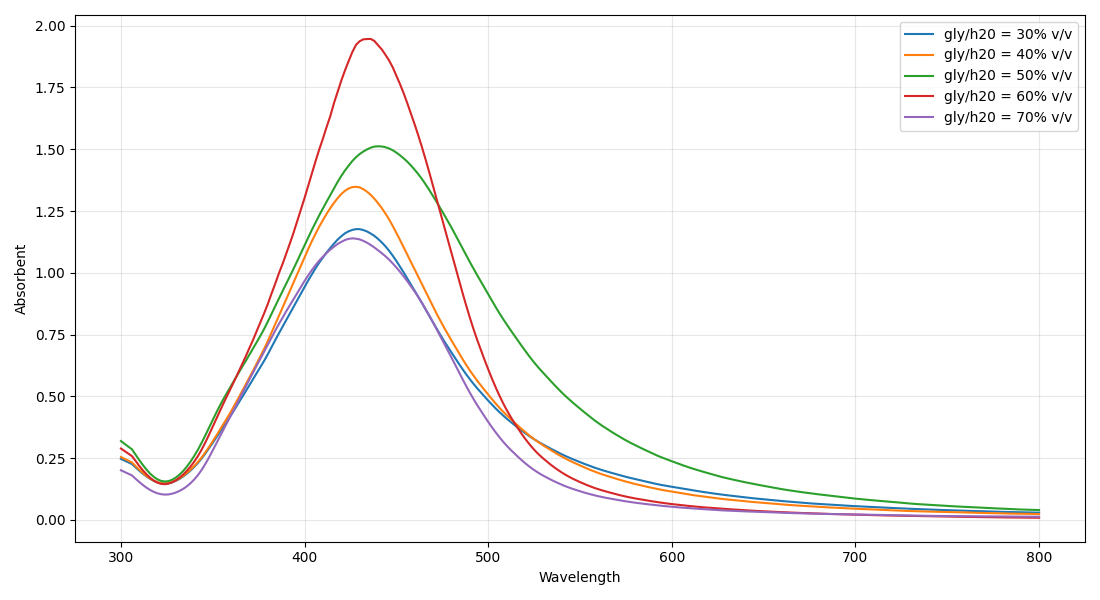
\includegraphics[width=0.95\textwidth]{figures/pvp_gly.png}
  \caption{Phổ UV--Vis của hệ Ag@PVP tại các tỷ lệ glycerol 30, 40, 50, 60 và 70\% (v/v).}
  \label{fig:pvp-glycerol}
\end{figure}

\subsection{Khảo sát ảnh hưởng của nồng độ NaOH}
Hình~\ref{fig:pvp-naoh} trình bày phổ UV--Vis của hệ Ag@PVP tại các nồng độ NaOH 0; 1,0; 1,5; 2,0; 2,5 và 3,0 mM.
Kết quả được sử dụng để đánh giá vai trò của điều kiện kiềm đối với sự hình thành và đặc trưng quang học của AgNPs.

\begin{figure}[htbp]
  \centering
  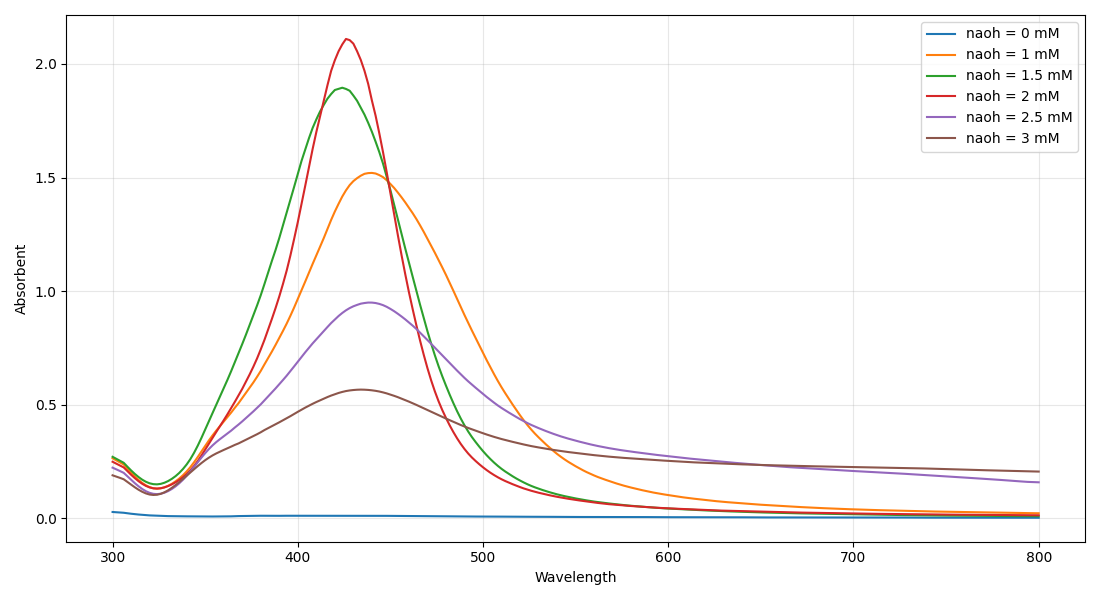
\includegraphics[width=0.95\textwidth]{figures/pvp_naoh.png}
  \caption{Phổ UV--Vis của hệ Ag@PVP tại các nồng độ NaOH 0; 1,0; 1,5; 2,0; 2,5 và 3,0 mM.}
  \label{fig:pvp-naoh}
\end{figure}

\subsection{Khảo sát ảnh hưởng của nhiệt độ phản ứng}
Hình~\ref{fig:pvp-temperature} trình bày phổ UV--Vis của hệ Ag@PVP khi nhiệt độ phản ứng được khảo sát tại 40, 50, 60, 70 và 80~$^\circ$C.
Sự thay đổi dải SPR theo nhiệt độ được xem xét cùng với các tiêu chí lựa chọn điều kiện phù hợp của hệ.

\begin{figure}[htbp]
  \centering
  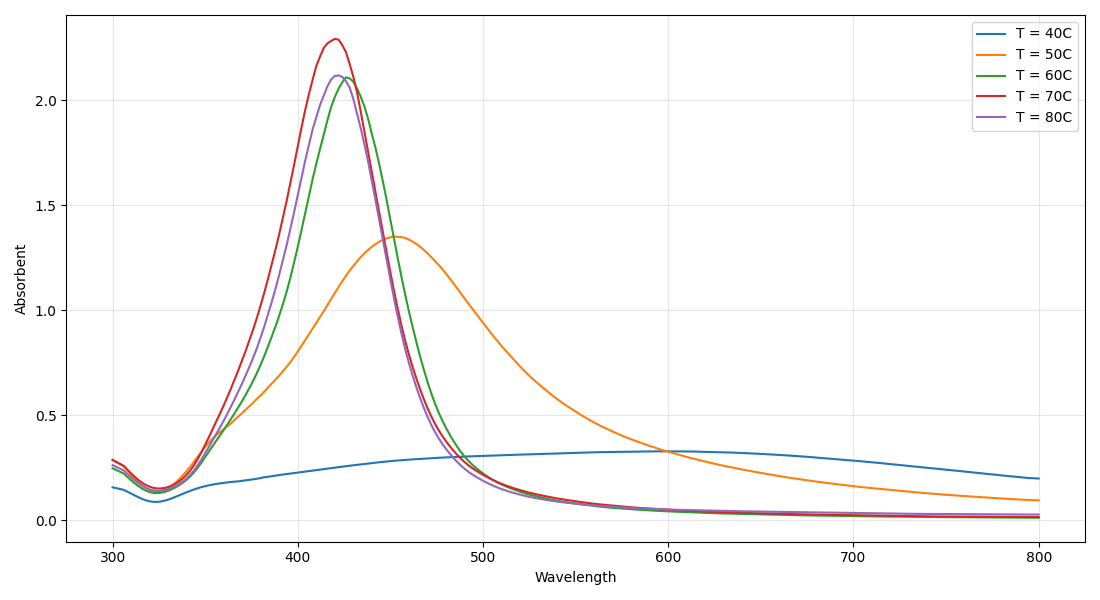
\includegraphics[width=0.95\textwidth]{figures/pvp_temp.png}
  \caption{Phổ UV--Vis của hệ Ag@PVP tại các nhiệt độ phản ứng 40, 50, 60, 70 và 80~$^\circ$C.}
  \label{fig:pvp-temperature}
\end{figure}

\subsection{Khảo sát ảnh hưởng của thời gian phản ứng}
Hình~\ref{fig:pvp-time} trình bày phổ UV--Vis của hệ Ag@PVP tại các thời điểm 5, 10, 15, 20, 25, 30 và 35 phút.
Các phổ được sử dụng để theo dõi diễn biến hình thành AgNPs theo thời gian phản ứng.

\begin{figure}[htbp]
  \centering
  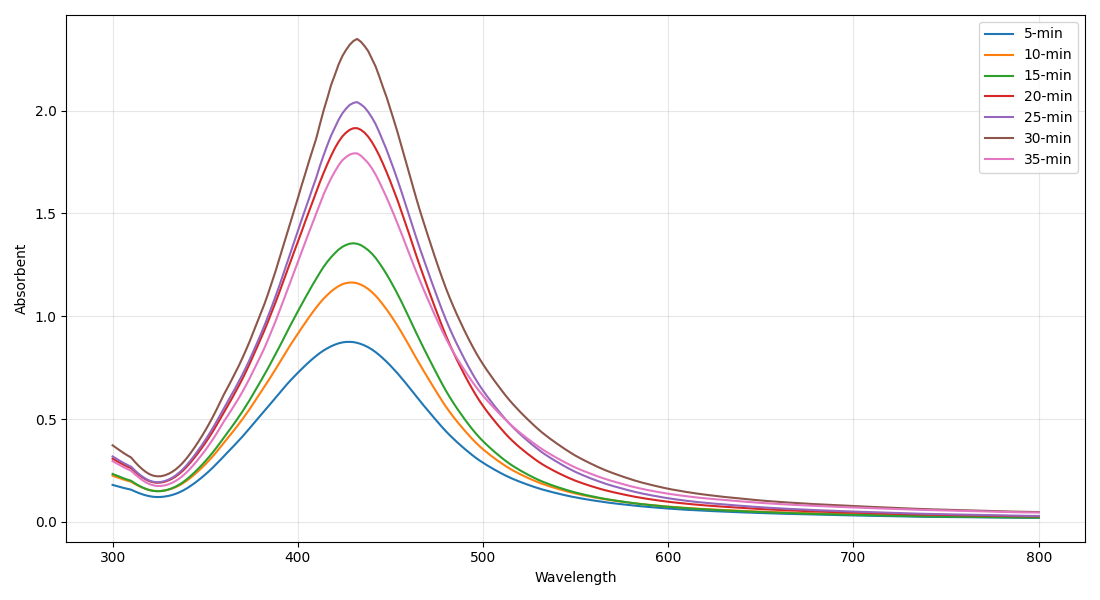
\includegraphics[width=0.95\textwidth]{figures/pvp_time.png}
  \caption{Phổ UV--Vis của hệ Ag@PVP tại các thời gian phản ứng 5, 10, 15, 20, 25, 30 và 35 phút.}
  \label{fig:pvp-time}
\end{figure}

\subsection{Khảo sát ảnh hưởng của nồng độ PVP}
Hình~\ref{fig:pvp-concentration} trình bày phổ UV--Vis của hệ Ag@PVP khi nồng độ PVP được khảo sát tại 0; 1; 2; 3 và 4\% (w/v).
Mẫu không bổ sung PVP được sử dụng làm đối chứng để đánh giá vai trò của polymer bảo vệ đối với trạng thái phân tán và đáp ứng quang học của AgNPs.

\begin{figure}[htbp]
  \centering
  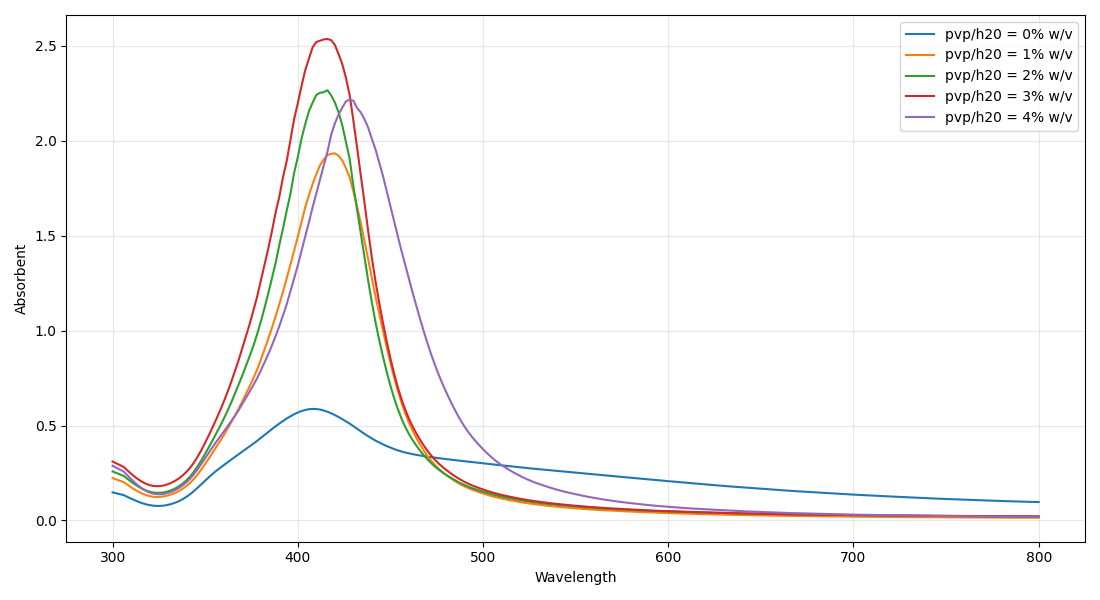
\includegraphics[width=0.95\textwidth]{figures/pvp.png}
  \caption{Phổ UV--Vis của hệ Ag@PVP tại các nồng độ PVP 0; 1; 2; 3 và 4\% (w/v).}
  \label{fig:pvp-concentration}
\end{figure}

\section{Kết quả khảo sát OFAT đối với hệ Ag@CMC}
Kết quả khảo sát đơn yếu tố đối với hệ Ag@CMC được trình bày theo trình tự tỷ lệ glycerol, nồng độ NaOH, nhiệt độ phản ứng, thời gian phản ứng và nồng độ CMC.
Đối với từng khảo sát, các yếu tố không được thay đổi được giữ cố định theo điều kiện đã lựa chọn ở bước khảo sát trước đó.
Phổ UV--Vis được sử dụng để theo dõi sự xuất hiện, vị trí và cường độ của dải hấp thụ SPR.

\subsection{Khảo sát ảnh hưởng của tỷ lệ glycerol}
Hình~\ref{fig:cmc-glycerol} trình bày phổ UV--Vis của hệ Ag@CMC khi tỷ lệ glycerol được khảo sát tại 30, 40, 50, 60 và 70\% (v/v).
Sự thay đổi vị trí, cường độ và độ rộng của dải SPR được sử dụng để đánh giá ảnh hưởng của tỷ lệ glycerol đến quá trình hình thành AgNPs.

\begin{figure}[htbp]
  \centering
  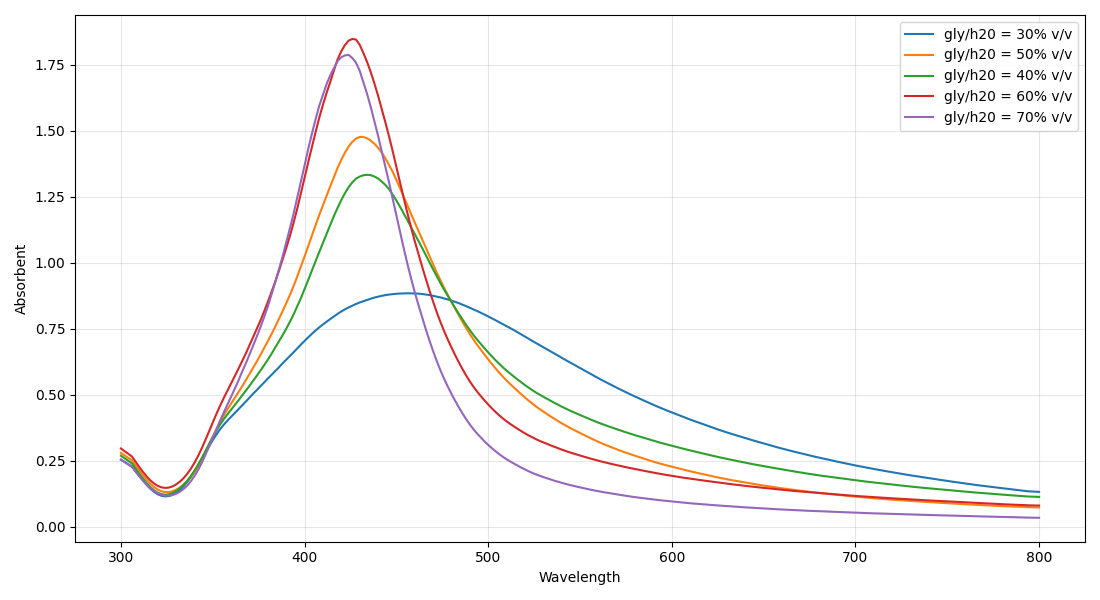
\includegraphics[width=0.95\textwidth]{figures/cmc_gly.png}
  \caption{Phổ UV--Vis của hệ Ag@CMC tại các tỷ lệ glycerol 30, 40, 50, 60 và 70\% (v/v).}
  \label{fig:cmc-glycerol}
\end{figure}

\subsection{Khảo sát ảnh hưởng của nồng độ NaOH}
Hình~\ref{fig:cmc-naoh} trình bày phổ UV--Vis của hệ Ag@CMC tại các nồng độ NaOH 1, 2, 3 và 4 mM.
Kết quả được sử dụng để đánh giá vai trò của điều kiện kiềm đối với sự hình thành và đặc trưng quang học của AgNPs.

\begin{figure}[htbp]
  \centering
  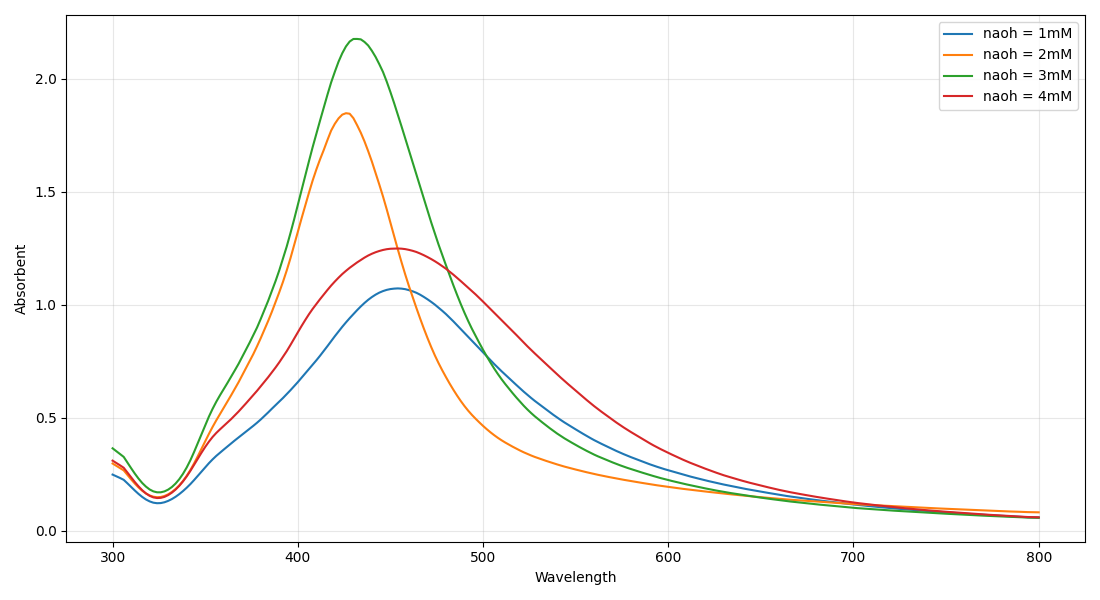
\includegraphics[width=0.95\textwidth]{figures/cmc_naoh.png}
  \caption{Phổ UV--Vis của hệ Ag@CMC tại các nồng độ NaOH 1, 2, 3 và 4 mM.}
  \label{fig:cmc-naoh}
\end{figure}

\subsection{Khảo sát ảnh hưởng của nhiệt độ phản ứng}
Hình~\ref{fig:cmc-temperature} trình bày phổ UV--Vis của hệ Ag@CMC khi nhiệt độ phản ứng được khảo sát tại 40, 50, 60, 70 và 80~$^\circ$C.
Sự thay đổi dải SPR theo nhiệt độ được xem xét cùng với các tiêu chí lựa chọn điều kiện phù hợp của hệ.

\begin{figure}[htbp]
  \centering
  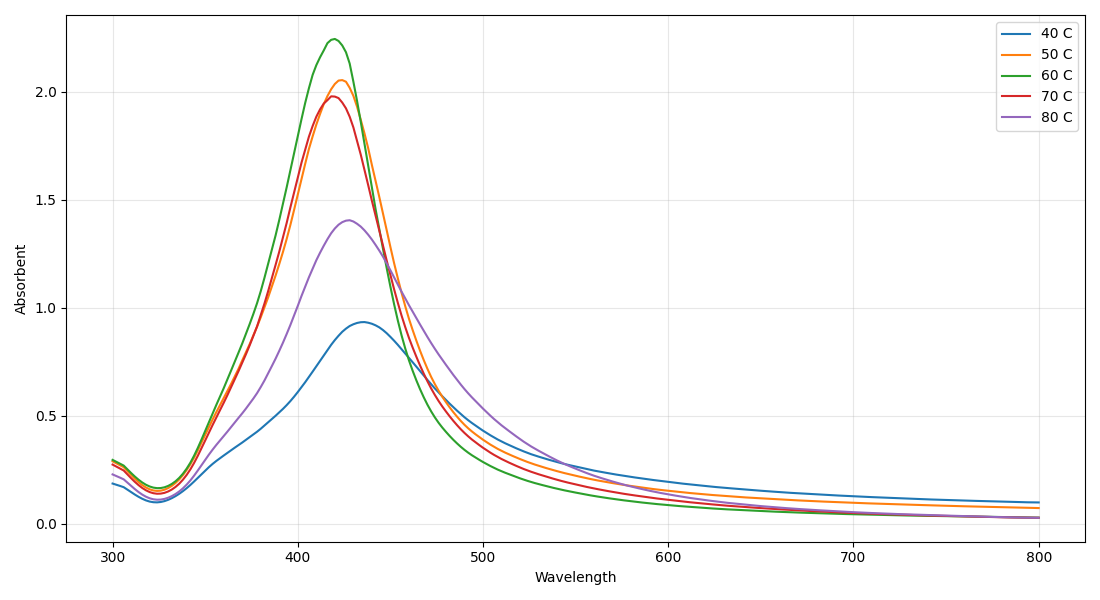
\includegraphics[width=0.95\textwidth]{figures/cmc_temp.png}
  \caption{Phổ UV--Vis của hệ Ag@CMC tại các nhiệt độ phản ứng 40, 50, 60, 70 và 80~$^\circ$C.}
  \label{fig:cmc-temperature}
\end{figure}

\subsection{Khảo sát ảnh hưởng của thời gian phản ứng}
Hình~\ref{fig:cmc-time} trình bày phổ UV--Vis của hệ Ag@CMC tại các thời điểm 5, 10, 15, 20, 25 và 30 phút.
Các phổ được sử dụng để theo dõi diễn biến hình thành AgNPs theo thời gian phản ứng.

\begin{figure}[htbp]
  \centering
  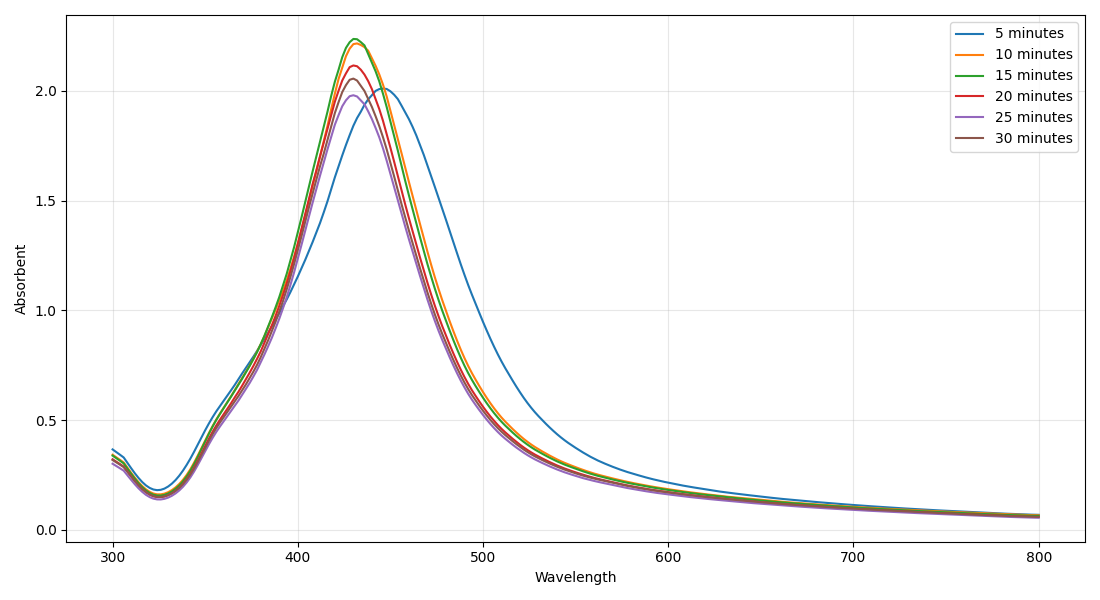
\includegraphics[width=0.95\textwidth]{figures/cmc_time.png}
  \caption{Phổ UV--Vis của hệ Ag@CMC tại các thời gian phản ứng 5, 10, 15, 20, 25 và 30 phút.}
  \label{fig:cmc-time}
\end{figure}

\subsection{Khảo sát ảnh hưởng của nồng độ CMC}
Hình~\ref{fig:cmc-concentration} trình bày phổ UV--Vis của hệ Ag@CMC khi nồng độ CMC được khảo sát tại 0,3; 0,6 và 0,9\% (w/v).
Các phổ này được sử dụng để đánh giá ảnh hưởng của hàm lượng CMC đến trạng thái phân tán và đáp ứng quang học của AgNPs.

\begin{figure}[htbp]
  \centering
  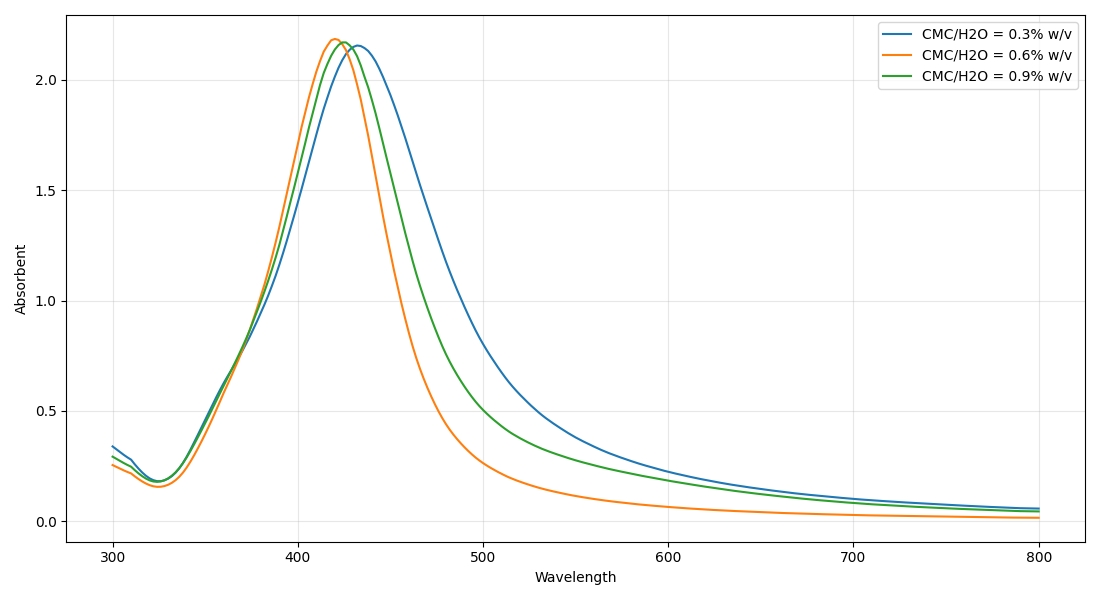
\includegraphics[width=0.95\textwidth]{figures/cmc.png}
  \caption{Phổ UV--Vis của hệ Ag@CMC tại các nồng độ CMC 0,3; 0,6 và 0,9\% (w/v).}
  \label{fig:cmc-concentration}
\end{figure}

\section{Đặc trưng AgNPs tại điều kiện tối ưu}
\subsection{Kích thước, phân bố kích thước và điện thế zeta}
Trình bày kết quả DLS và điện thế zeta của mẫu tối ưu; đối chiếu với tiêu chí đã đặt ra.

\subsection{Hình thái và cấu trúc vật liệu}
Trình bày ảnh TEM/SEM, giản đồ XRD và phổ FTIR của mẫu tối ưu. Thảo luận kích thước thực, hình dạng, pha tinh thể và tương tác bề mặt.

\section{So sánh hiệu quả bảo vệ hạt của PVP và CMC}
\subsection{Ảnh hưởng đến quá trình hình thành AgNPs}
So sánh màu sắc, phổ UV-Vis và tốc độ hình thành hạt ở hai hệ PVP và CMC trong cùng điều kiện phản ứng.

\subsection{Ảnh hưởng đến kích thước và hình thái hạt}
So sánh kết quả DLS, TEM/SEM và chỉ số đa phân tán để đánh giá khả năng kiểm soát kích thước của mỗi capping agent.

\subsection{Đánh giá độ ổn định theo thời gian}
Theo dõi sự thay đổi phổ UV-Vis, kích thước và điện thế zeta trong thời gian bảo quản đã lựa chọn.

\subsection{Đánh giá độ ổn định theo pH, nhiệt độ và lực ion}
So sánh độ bền của hai hệ khi thay đổi pH, nhiệt độ hoặc nồng độ muối điện ly. Xác định điều kiện gây kết tụ hoặc mất ổn định rõ rệt.

\subsection{Thảo luận cơ chế bảo vệ}
Diễn giải kết quả dựa trên cơ chế cản trở không gian của PVP và cơ chế ổn định điện tích của CMC. Liên hệ điện thế zeta, dữ liệu FTIR và khả năng chống kết tụ để rút ra nhận định.

\section{Tổng hợp kết quả thảo luận}
Tóm tắt các thông số tối ưu, đặc trưng AgNPs thu được và chất bảo vệ phù hợp theo từng tiêu chí đánh giá.

\chapter{Kết luận và hướng phát triển}

\section{Kết luận}
Tóm tắt đóng góp chính của luận văn.

\section{Hạn chế}
Nêu các hạn chế còn tồn tại.

\section{Hướng phát triển}
Đề xuất các hướng nghiên cứu tiếp theo.


\appendix
\chapter{Biểu mẫu số liệu thực nghiệm}

\section{Điều kiện tổng hợp AgNPs}
Đặt bảng số liệu gốc cho các thí nghiệm khảo sát nồng độ AgNO$_3$, nhiệt độ, thời gian, tỉ lệ glycerol/nước, tốc độ khuấy và nồng độ capping agent.

\section{Kết quả đặc trưng hóa}
Đặt bảng số liệu UV-Vis, DLS, điện thế zeta, XRD, FTIR và ảnh TEM/SEM bổ sung.

\section{Kết quả thử độ ổn định}
Đặt số liệu theo dõi độ ổn định theo thời gian, pH, nhiệt độ và lực ion cho các hệ PVP và CMC.


\end{document}
